\documentclass{article}

\usepackage{tabu}
\usepackage{pbox}
\usepackage[margin=1in]{geometry}
\usepackage{xcolor}
\usepackage{amsmath}
\usepackage{graphicx}

\frenchspacing
\setlength{\parskip}{1em}
\renewcommand{\arraystretch}{1.5}
\setlength\parindent{0pt}

\begin{document}

\section{MOSFETs}

Definitions:

\vspace{-5mm}
\begin{itemize} \itemsep0pt
	\item \(k_n \equiv \mu_nC_{ox} \frac{W}{L}\), \(k_p \equiv \mu_pC_{ox} \frac{W}{L}\)
	\item \(k'_n \equiv \mu_nC_{ox}\), \(k'_p \equiv \mu_pC_{ox}\)
	\item \(V_{OV} \equiv V_{GS}-V_{th}\)
	\item \(V_A \equiv \frac{1}{\lambda}\)
	\item \(V'_A \equiv \frac{V_A}{L}\)
	\item \(g_m \equiv \frac{\partial i_D}{\partial v_{GS}} = \frac{i_d}{v_{gs}}\)
\end{itemize}

Large signal characteristics, \(k=k_n\) or \(k_p\) as appropriate:

\begin{tabu}{  l  X  X  }
	\hline
	Region & Condition & Properties \\ \hline
	Saturation & \(|V_{GS}| > |V_{th}| \bigwedge |V_{DS}| \geq |V_{OV}|\) &
	\pbox{20cm}{
		\vspace{1mm}
		\(\begin{aligned}
					I_D &= \frac{k}{2} V_{OV}^2 (1+\frac{V_{DS}}{|V_A|}) \\
			   &\approx \frac{k}{2} V_{OV}^2
		\end{aligned}\)
	}\\

	Triode & \(|V_{GS}| > |V_{th}| \bigwedge |V_{DS}| \leq |V_{OV}|\) &
	\pbox{20cm}{ \(I_D = k(|V_{OV}|-\frac{1}{2}|V_{DS}|)|V_{DS}|\) } \\

	Cutoff & \(|V_{GS}| \leq |V_{th}|\) & \(I_D = 0\)\\
	\hline
\end{tabu}

For N-channel devices, all absolute value operations can be ignored.

\vspace{5mm}
Small signal characteristics (saturation only):

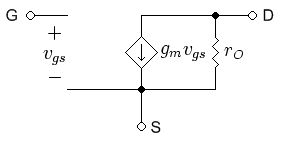
\includegraphics[height=100pt]{MOSFET_Small_Signal.png}\footnote{Image by Brews ohare at English Wikipedia} % https://commons.wikimedia.org/wiki/File:MOSFET_Small_Signal.png

\vspace{-5mm}
\begin{itemize}
	\item \(g_m = \frac{2I_D}{V_{OV}} = k|V_{OV}|\)
	\item \(r_o = \frac{V_A}{I_D}\)
\end{itemize}

\end{document}
